\section{Docker \& Kubernetes}
\label{sec:docker-kubernetes}
Το \emph{Docker}\footnote{\url{https://www.docker.com/}} είναι μία ανοιχτή πλατφόρμα για ανάπτυξη και εκτέλεση εφαρμογών και δίνει τη δυνατότητα διαχωρισμού της εφαρμογής που εκτελείται από το υπόλοιπο σύστημα. Αυτό επιτυγχάνεται με τη χρήση των κιβωτίων (\emph{containers}). Τα \emph{containers}, είναι τελείως αυτόνομες εφαρμογές ανεξάρτητες από το υπόλοιπο σύστημα.

Το \emph{Kubernetes}\footnote{\url{https://kubernetes.io/}} είναι μία φορητή, επεκτάσιμη πλατφόρμα ανοιχτού λογισμικού για τη διαχείριση φόρτου εργασίας και υπηρεσιών με \emph{containers}.

Στα πλαίσια της διπλωματικής εργασίας η βάση δεδομένων αποτελεί ένα \emph{docker container} και το εργαλείο \emph{RASA-X} ένα σύμπλεγμα από \emph{containers} το οποίο είναι προσβάσιμο μέσω του \emph{Kubernetes}. Στο \autoref{fig:docker-containers} παρουσιάζεται η βασική δομή του \emph{Docker}.

\begin{figure}[!ht]
  \centering
  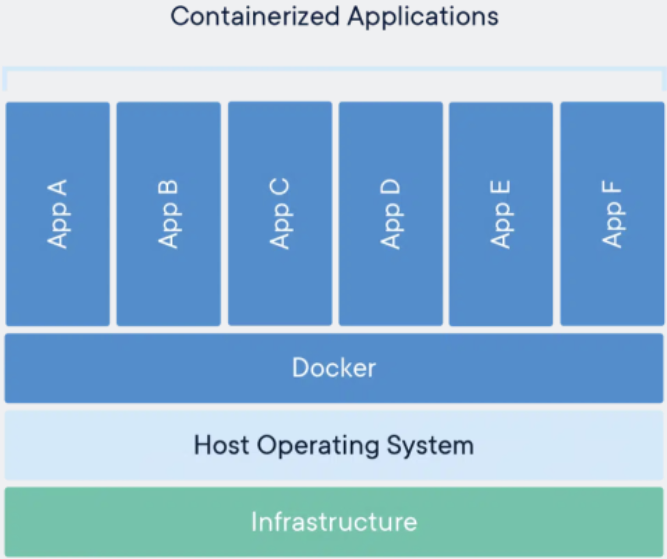
\includegraphics[width=0.7\textwidth]{images/chapter3/docker-containerized-applictions.png}
  \captionsetup{justification=centering}
  \captionsource{Βασική δομή \emph{Dokcer}}{\url{https://www.docker.com/resources/what-container}}
  \label{fig:docker-containers}
\end{figure}
\noindent